% Problem 1 - Residential Power Distribution Mesh Analysis (24 points)
\Point{residentialpower}{load_estimate}{2}
\Point{residentialpower}{meshanalysis}{12}
\Point{residentialpower}{openneutral}{10}
\Point{residentialpower}{deviceimpact}{2}
\begin{mainquestion}{residentialpower}{Mesh Analysis}
The DC equivalent circuit of a simple residential power distribution is shown below. $R_{w}$ represents the hot wire (typically black) resistance, and $R_{n}$ represents the neutral wire (typically white) resistance. The other resistances represent loads that are drawing power.

\begin{center}
    \includegraphics[width=4in]{../v0/circuit.png}
\end{center}

\begin{partquestion}{load_estimate}
{$R_{1}$ models a heavy duty \qty{2.88}{\kilo\watt} microwave built to run on 120V. \\ $R_{2}$ models a \qty{1.2}{\kilo\watt} blender that draws 10A when crunching ice. \\ $R_{3}$ models a 240V stovetop that draws $\approx\qty{18.5}{\ampere}$ with two of its burners on. \\
Find $R_1$, $R_2$ and $R_3$ to the nearest ohm.}

\begin{answer}
    We can use Ohm's law and the definition of power to find the resistance for each load.
    \[P = \frac{V^2}{R_1} \hspace{1cm} R_1=\frac{120^2}{2880}=5\Omega\]
    \[P = I^2R_2 \hspace{1cm} R_2=\frac{1200}{10^2}=12\Omega\]
    \[R_3 = \frac{V}{I}=\frac{240}{18.5}=13\Omega\]
\end{answer}
\end{partquestion}

\begin{partquestion}{meshanalysis}{Using your results from part (\cref{prob:residentialpower:load_estimate}), use mesh analysis to determine the voltage across each of the three loads given $R_{w}=R_{n}=0.2~\Omega$.}
\begin{answer}
Create three mesh loops in the clockwise direction for the three currents $i_{1}$ in the top-left loop, $i_{2}$ in the bottom-left loop, and $i_{3}$ in the right-hand loop. Using KVL around each loop gives:

\begin{gather*}
R_w i_1 + R_1 (i_1 - i_3) + R_n (i_1 - i_2) = 120 \\
R_w i_2 + R_2 (i_2 - i_3) + R_n (i_2 - i_1) = 120 \\
R_3 i_3 + R_1 (i_3 - i_1) + R_2 (i_3 - i_2) = 0
\end{gather*}

Then we gather like terms:

\begin{gather*}
(R_w + R_1 + R_n)i_1 - R_n i_2 - R_1 i_3 = 120 \\
- R_n i_1 + (R_w + R_2 + R_n)i_2 - R_2 i_3 = 120 \\
- R_1 i_1 - R_2 i_2 + (R_1 + R_2 + R_3)i_3 = 0
\end{gather*}

And this can be neatly written as a matrix:

\[
\begin{bmatrix}
R_w + R_1 + R_n & -R_n & -R_1 \\
-R_n & R_w + R_2 + R_n & -R_2 \\
-R_1 & -R_2 & R_3 + R_1 + R_2
\end{bmatrix}
\begin{bmatrix}
i_1 \\
i_2 \\
i_3
\end{bmatrix}
=
\begin{bmatrix}
120 \\
120 \\
0
\end{bmatrix}
\]

Substituting the given values produces:

\[
\begin{bmatrix}
5.4 & -0.2 & -5 \\
-0.2 & 12.4 & -12 \\
-5 & -12 & 30
\end{bmatrix}
\begin{bmatrix}
i_1 \\
i_2 \\
i_3
\end{bmatrix}
=
\begin{bmatrix}
120 \\
120 \\
0
\end{bmatrix}
\]

This can be solved quickly in MATLAB using matrix inversion, or you can solve by hand. Multiply the second equation by 25 and subtract from the third equation to give:
\[-322i_2+330i_3=-3000\]
Multiply the second equation by 27 and add to the first equation to give:
\[334.6i_2-329i_3=3360\]
From these last two equations, we can eliminate $i_3$ by multiplying the first by 329 and the second by 330 and adding the results.  We get:
\[4480i_2 = 121800\]\[i_2 = \frac{435}{16}\unit{\ampere}\]
	  
Plugging this result back into either previous equation gives \[i_3=\frac{279}{16}\unit{\ampere}\] We can then solve for the first loop current using any of the three original equations, and it is calculated that \[i_1=\frac{315}{8}\unit{\ampere}\] 
In summary:
\begin{align*}
    i_1 &= \frac{315}{8} \approx \qty{39.4}{\ampere}\\
    i_2 &= \frac{435}{16} \approx \qty{27.2}{\ampere}\\
    i_3 &= \frac{279}{16} \approx \qty{17.4}{\ampere}
\end{align*}

The voltages across the three loads are then:
\begin{align*}
v_{1} &= (i_{1}-i_{3}) R_{1} = \left( \frac{315}{8} - \frac{279}{16} \right) 5 = \frac{1755}{16} \approx 109.7~\text{V} \\
v_{2} &= (i_{2}-i_{3}) R_{2} = \left( \frac{435}{16} - \frac{279}{16} \right) 12 = 117~\text{V} \\
v_{3} &= i_{3} R_{3} = \frac{279}{16} \cdot 13 = \frac{3627}{16} \approx 226.7~\text{V}
\end{align*}
\end{answer}
\end{partquestion}

\begin{partquestion}{openneutral}{If a wiring fault occurs such that the neutral becomes an open circuit, recalculate the voltages across the loads.}
\begin{answer}
With the neutral open, $R_{n}\to\infty$ and the left-hand and right-hand loops remain. Let $i_{1}$ be the clockwise current in the left loop and $i_{2}$ be the clockwise current in the right loop.

The KVL system becomes:
\begin{gather*}
R_wi_1 + (R_1 + R_2)(i_1 - i_2) + R_wi_1 = 240 \\
(R_1 + R_2)(i_2 - i_1) + R_3i_2 = 0
\end{gather*}

Gather like terms:
\begin{gather*}
(2R_w + R_1 + R_2)i_1 - (R_1 + R_2)i_2 = 240 \\
- (R_1 + R_2)i_1 + (R_1 + R_2 + R_3)i_2 = 0
\end{gather*}

As a matrix:
\[
\begin{bmatrix}
2R_w + R_1 + R_2 & -R_1 -R_2\\
-R_1 -R_2 & R_1 + R_2 + R_3
\end{bmatrix}
\begin{bmatrix}
i_1 \\
i_2
\end{bmatrix}
=
\begin{bmatrix}
240 \\
0
\end{bmatrix}
\]

Substituting values yields:
\[
\begin{bmatrix}
17.4 & -17\\
-17 & 30
\end{bmatrix}
\begin{bmatrix}
i_1 \\
i_2
\end{bmatrix}
=
\begin{bmatrix}
240 \\
0
\end{bmatrix}
\]

Solving gives $i_{2} = \frac{4080}{233} \approx 17.51~\text{A}$ and $i_{1} = \frac{7200}{233} \approx 30.90~\text{A}$. The load voltages are:
\begin{align*}
v_{1} &= (i_{1}-i_{2})R_1 = \frac{15600}{233} \approx 66.95~\text{V} \\
v_{2} &= (i_{1}-i_{2})R_2 = \frac{13337}{83} \approx 160.7~\text{V} \\
v_{3} &= i_{2} R_3 = \frac{19577}{86} \approx 227.6~\text{V}
\end{align*}
\end{answer}
\end{partquestion}

\begin{partquestion}{deviceimpact}{Suppose $R_2$ now represents a sensitive device. Postulate what might happen to it if it is plugged into this faulty circuit.}
\begin{answer}
Because $R_{2}$ now sees over 160 V instead of the expected 120 V, a sensitive device is likely to be exposed to an overvoltage condition. This can damage components, cause device failure, or lead to unsafe operation.
\end{answer}
\end{partquestion}

\end{mainquestion}


% Problem 2 - Superposition (10 points)
\clearpage
\Point{superposition}{calculatevab}{10}
\Point{superposition}{compare}{2}
\begin{mainquestion}{superposition}{Superposition}
Consider this circuit that you've solved in a previous assignment:

\begin{center}
    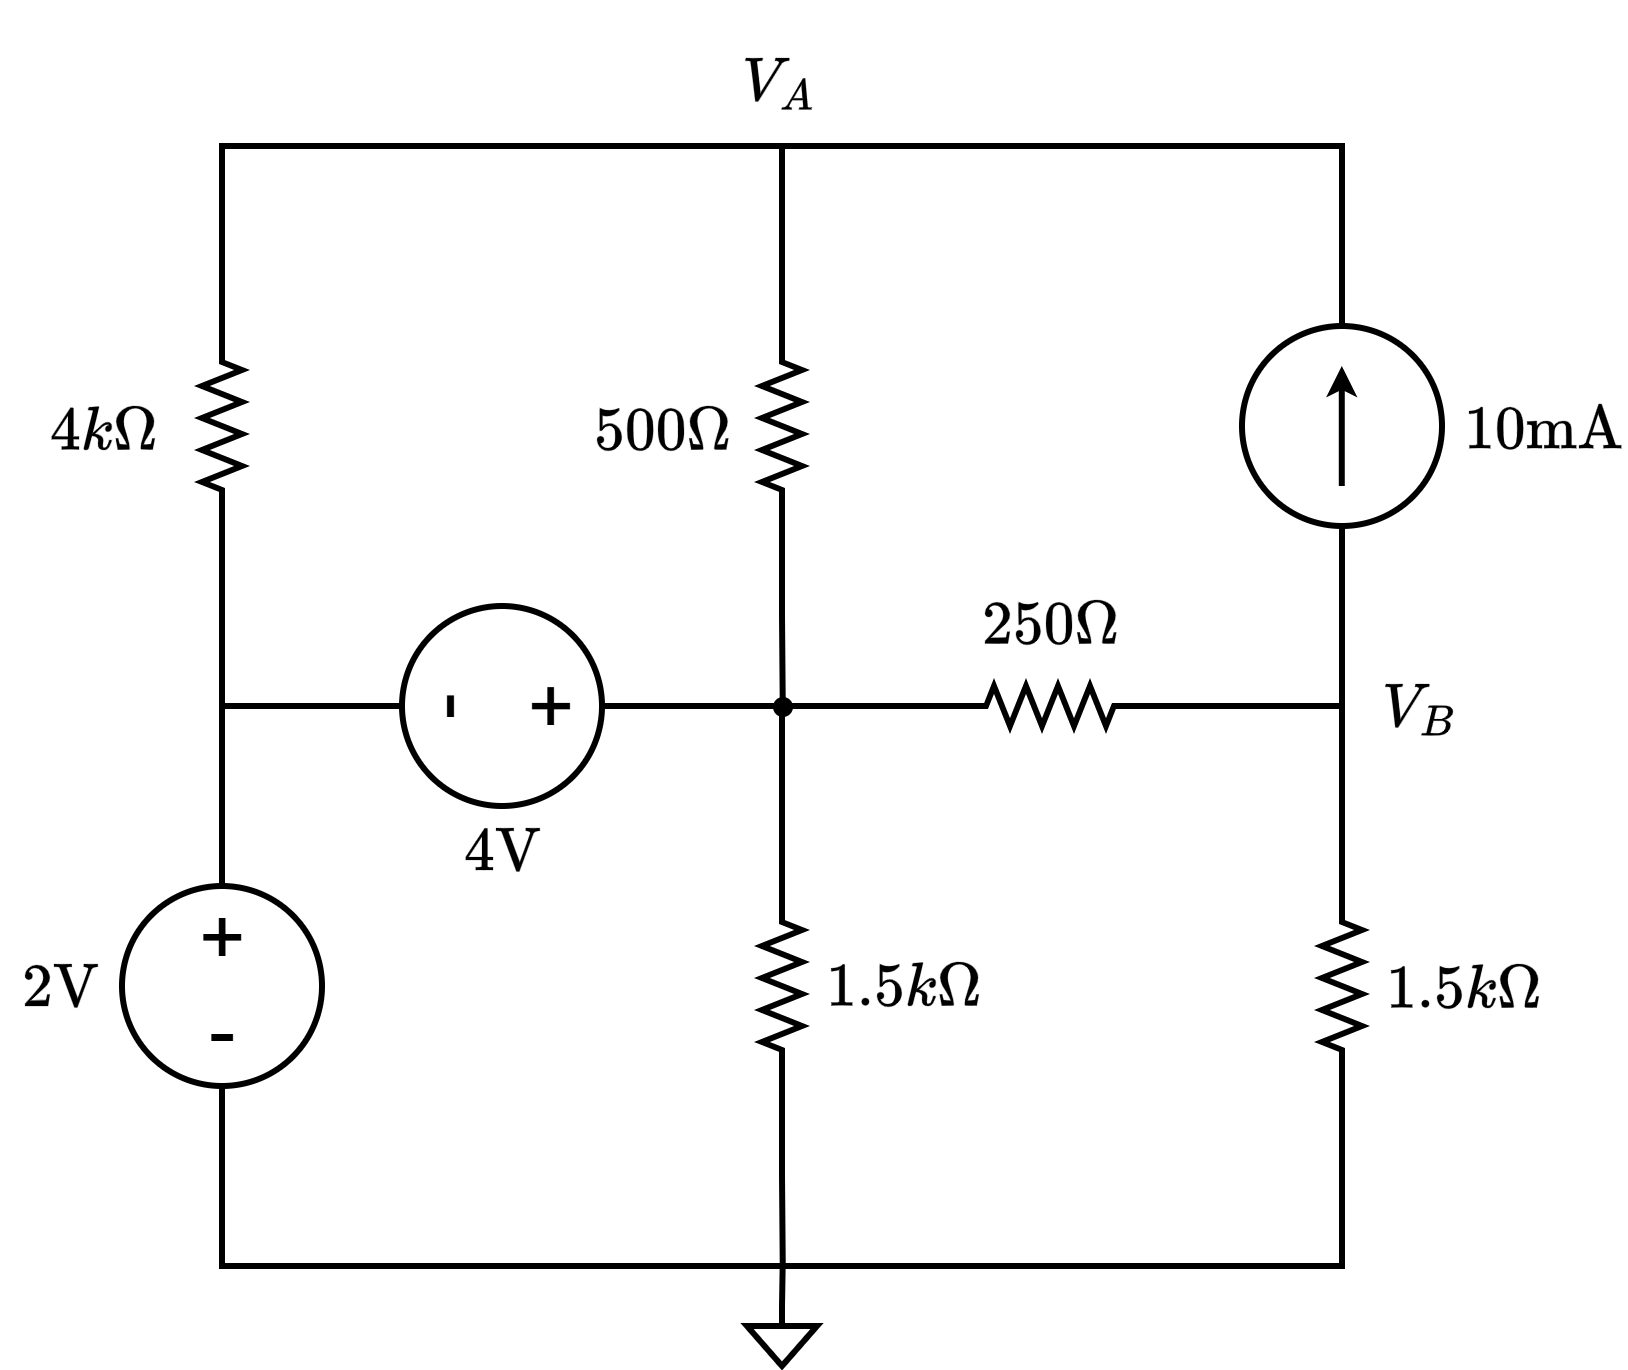
\includegraphics[width=0.8\textwidth]{questionbank/networks/superposition/v1/schematic.png}
\end{center}

\begin{partquestion}{calculatevab}{Use superposition to find $V_A$ and $V_B$.}
\begin{answer}
Superposition tells us that we can consider the effect of each independent source individually. We can do this by disabling all but one of the independent sources (open current sources, short voltage sources) and solving for the voltages at $V_A$ and $V_B$. Then we can add up the contributions to each and we should get the final values of $V_A$ and $V_B$, respectively.
\bigskip

\textbf{2V source only:} open the 10 mA source and short the 4 V source. The circuit becomes:
\begin{center}
    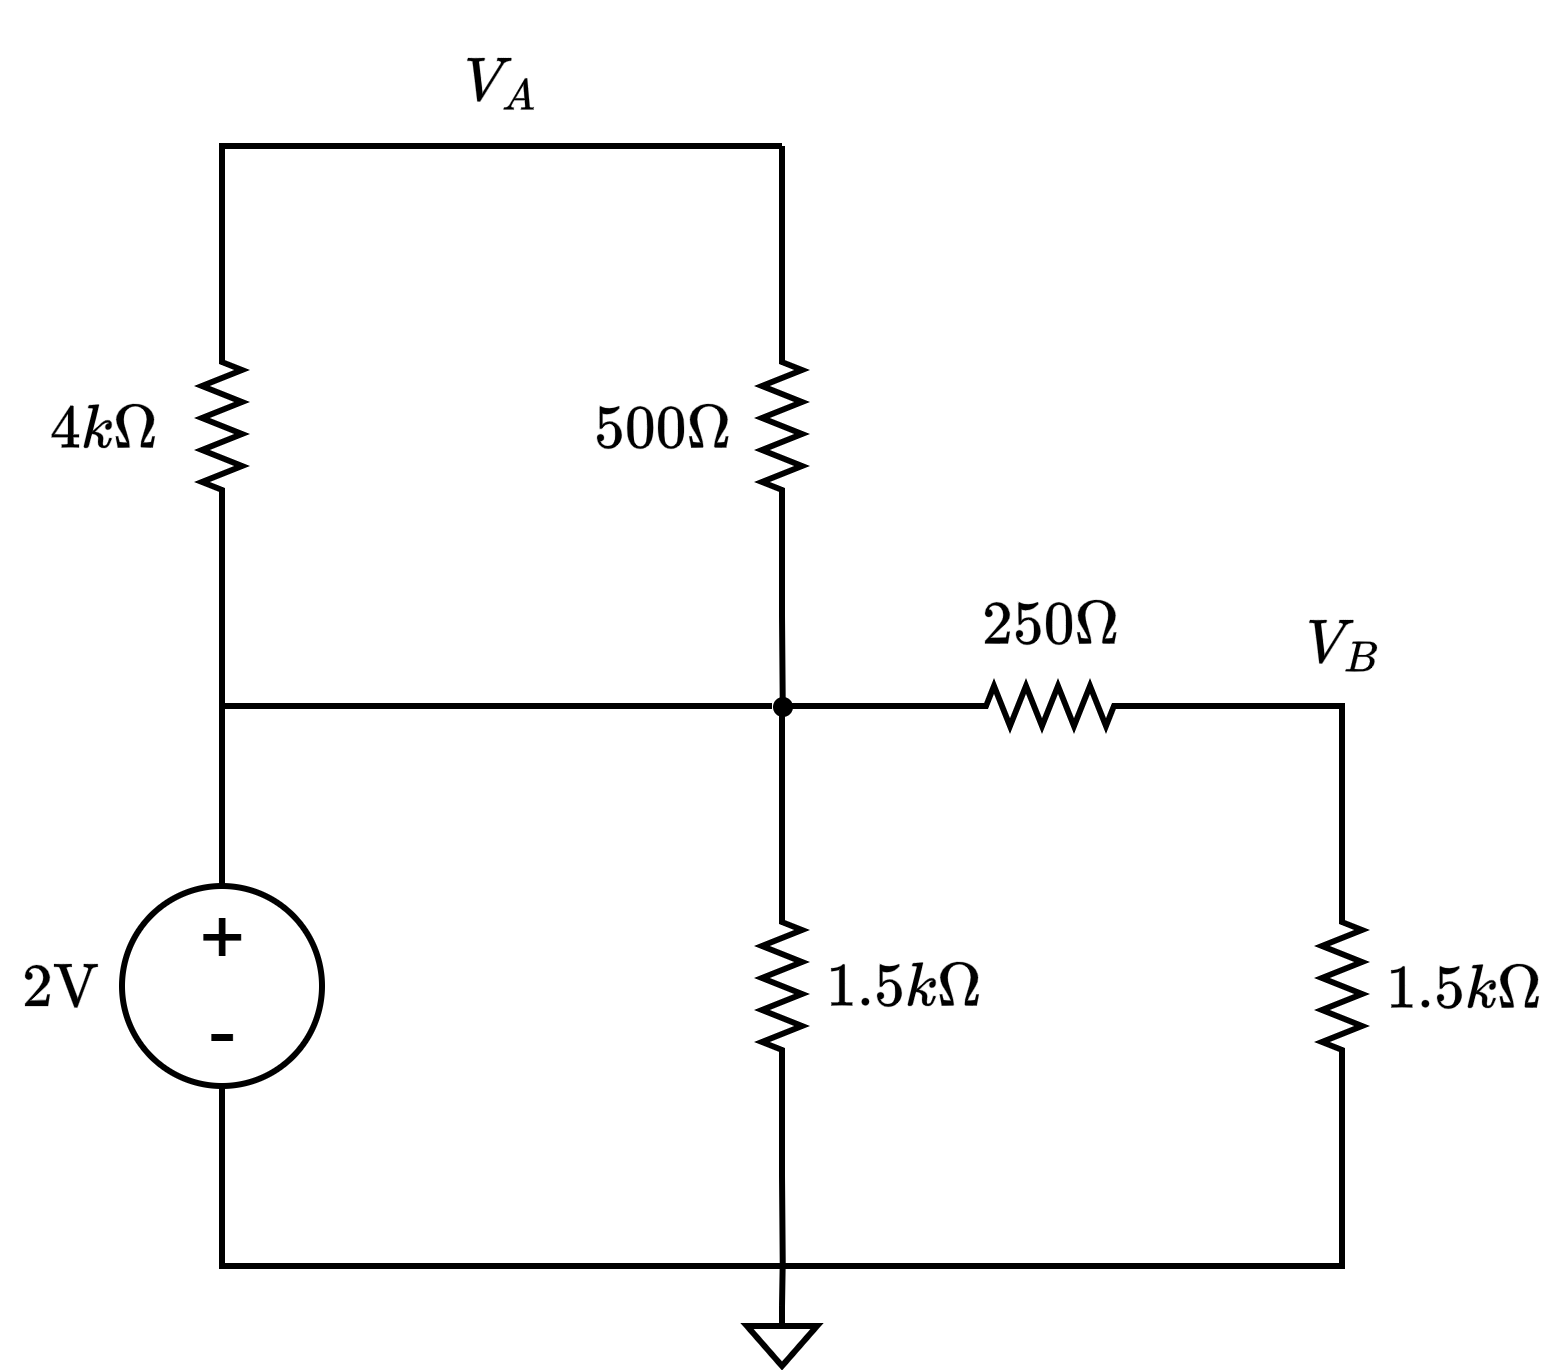
\includegraphics[width=0.6\textwidth]{questionbank/networks/superposition/v1/super_2v.png}
\end{center}

The circuit is now just a resistor network with a single independent source. We see right away that $V_B$ is the output of a voltage divider:
\[
V_B = 2\frac{1500}{1500 +250} = \frac{12}{7}\unit{\volt}
\]
$V_A$ is stranded at the top of the circuit. KVL tells us that the drop across the \qty{4}{\kilo\ohm} resistor and the \qty{500}{\ohm} must add up to zero, but parallel elements must have the same voltage:
\[
V_{4k\Omega} + V_{500\Omega} = 0 \hspace{1cm} V_{4k\Omega} = V_{500\Omega}
\]

The only solution is if $V_{4k\Omega}$ and $V_{500\Omega}$ are both \qty{0}{\volt}! This implies that $V_A$ is the same voltage as the voltage source, so:
\[V_A = \qty{2}{\volt}\]
\bigskip

\textbf{4 V source only:} open the 10 mA source and short the 2 V source. The circuit becomes:
\begin{center}
    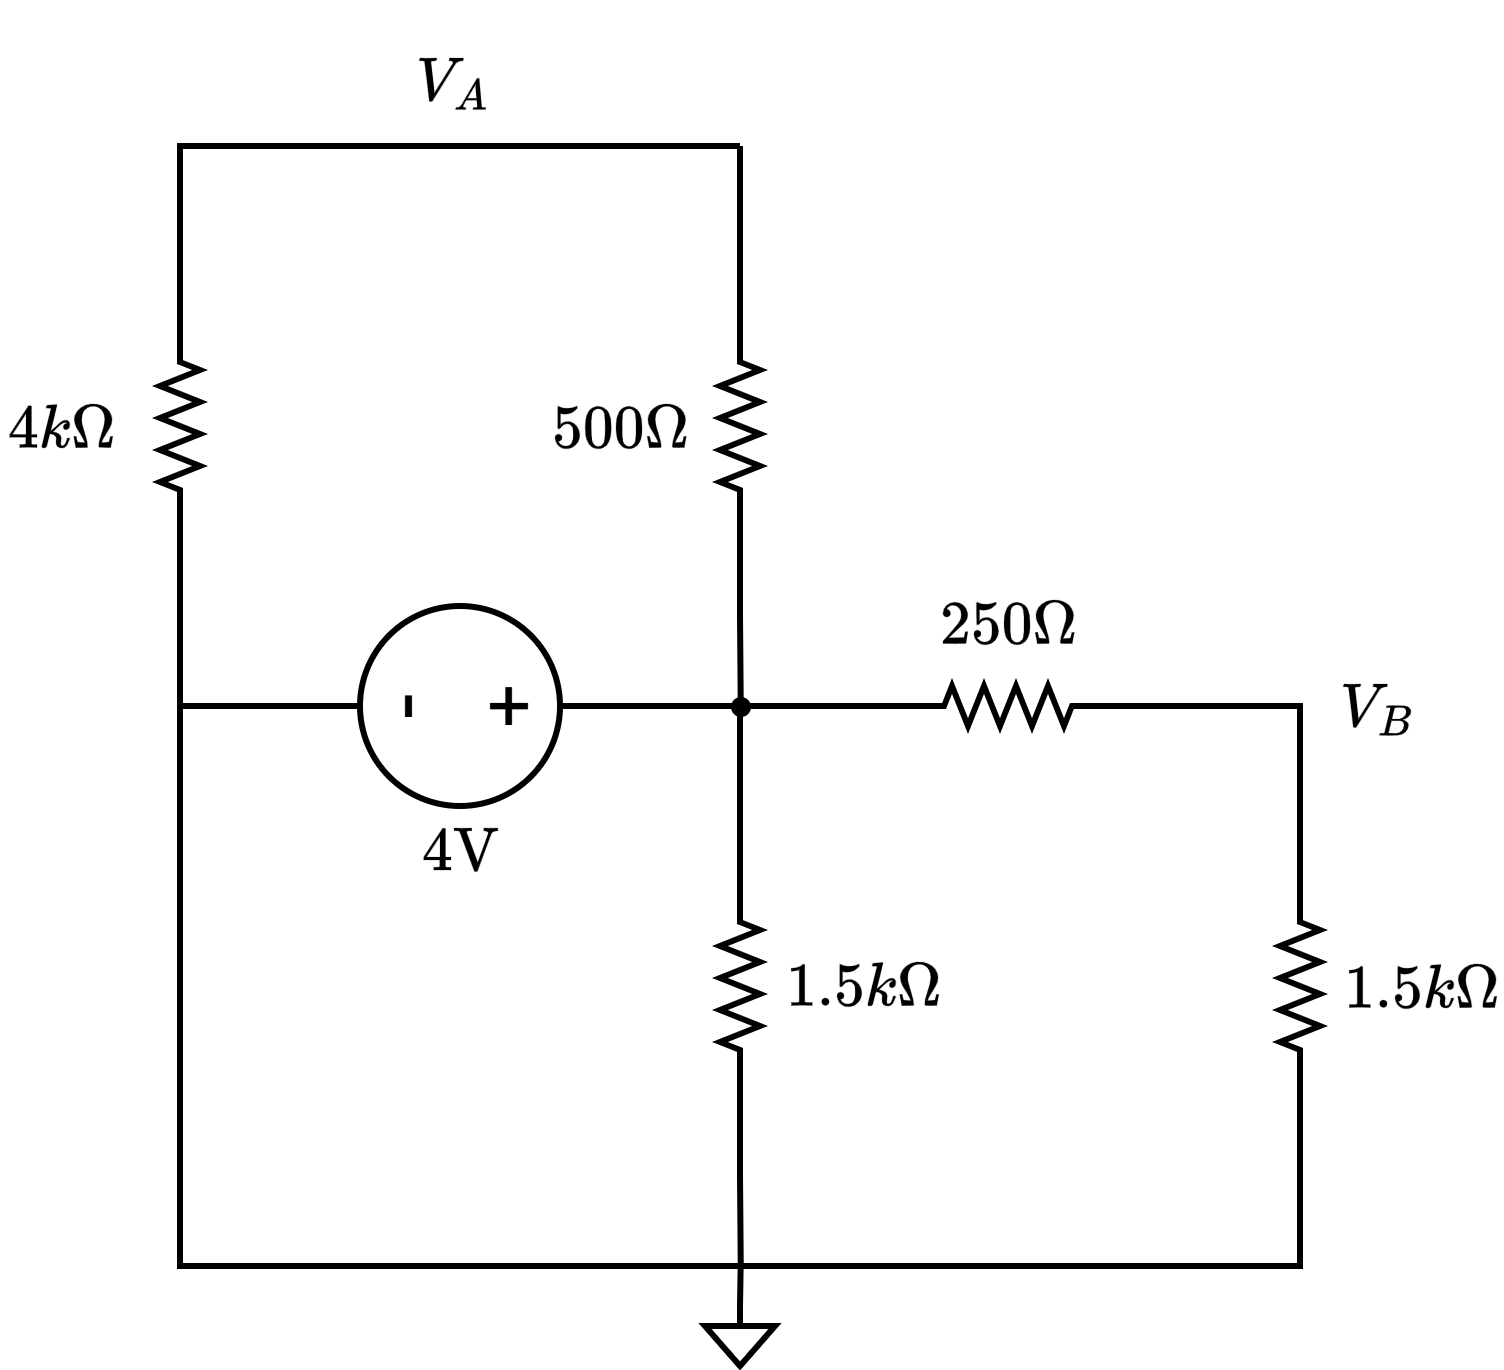
\includegraphics[width=3in]{questionbank/networks/superposition/v1/super_4v.png}
\end{center}

This is very similar to before, except now both $V_A$ and $V_B$ are voltage dividers:
\[
V_A = 4\frac{4000}{4000 +500} = \frac{32}{9}\unit{\volt}
\]

\[
V_B = 4\frac{1500}{1500 +250} = \frac{24}{7}\unit{\volt}
\]
\bigskip

\textbf{10 mA source only:} short both voltage sources. The circuit becomes:
\begin{center}
    \includegraphics[width=3in]{questionbank/networks/superposition/v1/super_10mA.png}
\end{center}

Let's take a second to figure out what we are looking at. The current from our 10mA source will pass through the \qty{4}{\kilo\ohm} resistor and the \qty{500}{\ohm} resistor in parallel before reaching ground. Then the current will pass through the \qty{1.5}{\kilo\ohm} resistor and the \qty{250}{\ohm} resistor in parallel on its way back to the current source. The other \qty{1.5}{\kilo\ohm} is shorted so the current won't bother to flow through it.

The voltages $V_A$ and $V_B$ will be the voltage drops across the effective parallel resistor pairs:

\[V_A = 10 \frac{0.5 \cdot 4}{4 + 0.5} = \frac{40}{9}\unit{\volt}\]
\[V_B = -10 \frac{0.25 \cdot 1.5}{1.5 + 0.25} = -\frac{15}{7}\unit{\volt}\]
Note $V_B$ is negative thanks to our passive sign convention.
\bigskip

Now we can sum our results to find the final values:
\[
V_A = 2 + \frac{32}{9} + \frac{40}{9} = \frac{90}{9} = \qty{10}{\volt}
\]
\[
V_B = \frac{12}{7} + \frac{24}{7} - \frac{15}{7} = \frac{21}{7} = \qty{3}{\volt}
\]
\end{answer}
\end{partquestion}

\begin{partquestion}{compare}{Does your result in part (\cref{prob:superposition:calculatevab}) match your solution from HW2 Problem 1? Which method do you prefer and why?}

\begin{answer}
    Our solution to HW2 Problem 1 found that the voltage across $R_5$ (rightmost \qty{1.5}{\kilo\ohm}) was \qty{3}{\volt} and the voltage across $R_1$ (upper right \qty{4}{\kilo\ohm}) was \qty{8}{\volt}. Given we assign the bottom node to be ground as shown, that would imply $V_A = 2 + 8 = \qty{10}{\volt}$ and $V_B = \qty{3}{\volt}$, a perfect match!
    In this case superposition made our job easier by removing the need to solve any systems of equations.
\end{answer}
\end{partquestion}

\end{mainquestion}


% Problem 3 - Ammeter Connection and Equivalent Circuits (16 points)
\clearpage
\Point{ammeter}{connection}{3}
\Point{ammeter}{thevenin}{5}
\Point{ammeter}{norton}{3}
\Point{ammeter}{ri300}{2}
\Point{ammeter}{ri0}{2}
\Point{ammeter}{rimax}{3}
\begin{mainquestion}{ammeter}{Equivalent Circuits}
Consider the circuit shown below. An ammeter with an internal resistance of $R_{i}$ is used to measure the current flowing through a 560$\Omega$ resistor between points $A$ and $B$.

\begin{center}
    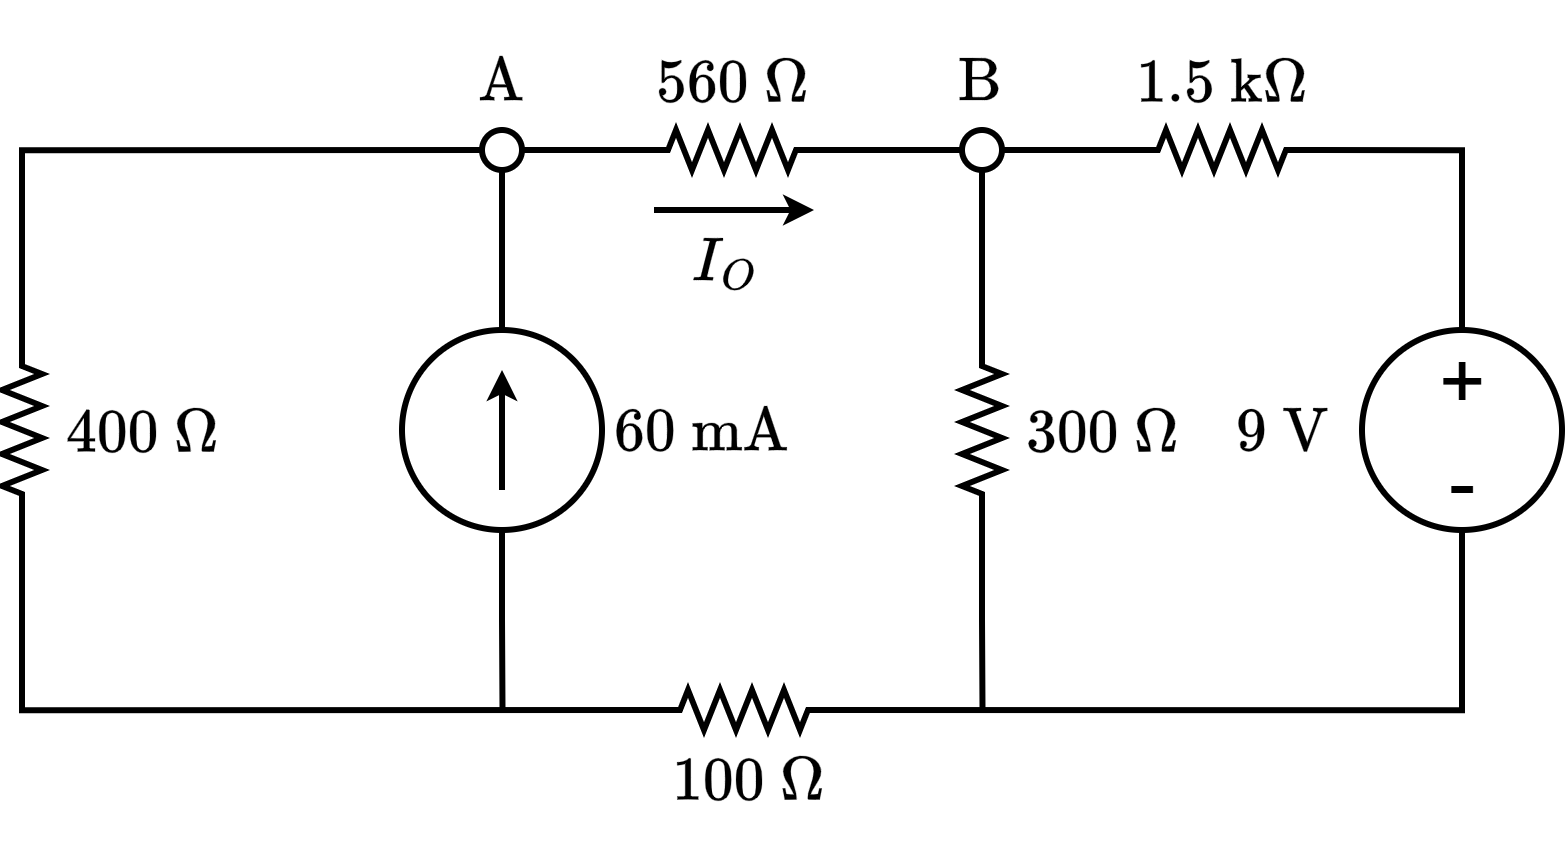
\includegraphics[width=5in]{questionbank/networks/ammeter_thevenin_norton/v1/circuit.png}
\end{center}

\begin{partquestion}{connection}{How should the ammeter be connected between $A$ and $B$? Show a sketch of the circuit (only include the portion between $A$ and $B$) which includes the ammeter with its internal resistance.}
\begin{answer}
The ammeter should be connected in series with the 560$\Omega$ resistor between terminals $A$ and $B$. This means the current through the load passes through the ammeter and its internal resistance.

\begin{center}
    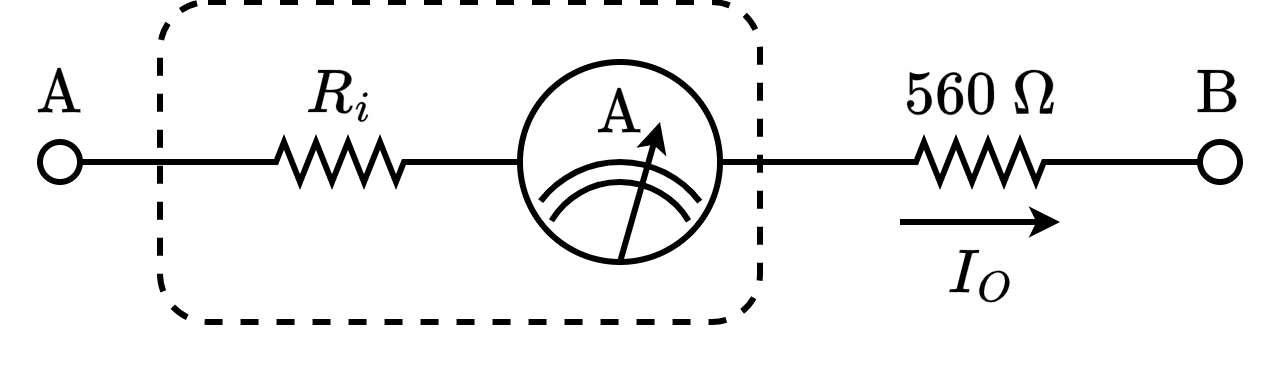
\includegraphics[width=0.7\textwidth]{questionbank/networks/ammeter_thevenin_norton/v1/ammeter_conn.png}
\end{center}
\end{answer}
\end{partquestion}

\begin{partquestion}{thevenin}{Find the Thévenin equivalent circuit at terminals $A$ and $B$ (without the 560$\Omega$ load).}
\begin{answer}
To find the Thévenin resistance, we zero out all independent sources. The current source becomes an open circuit and the voltage source becomes a short circuit:

\begin{center}
    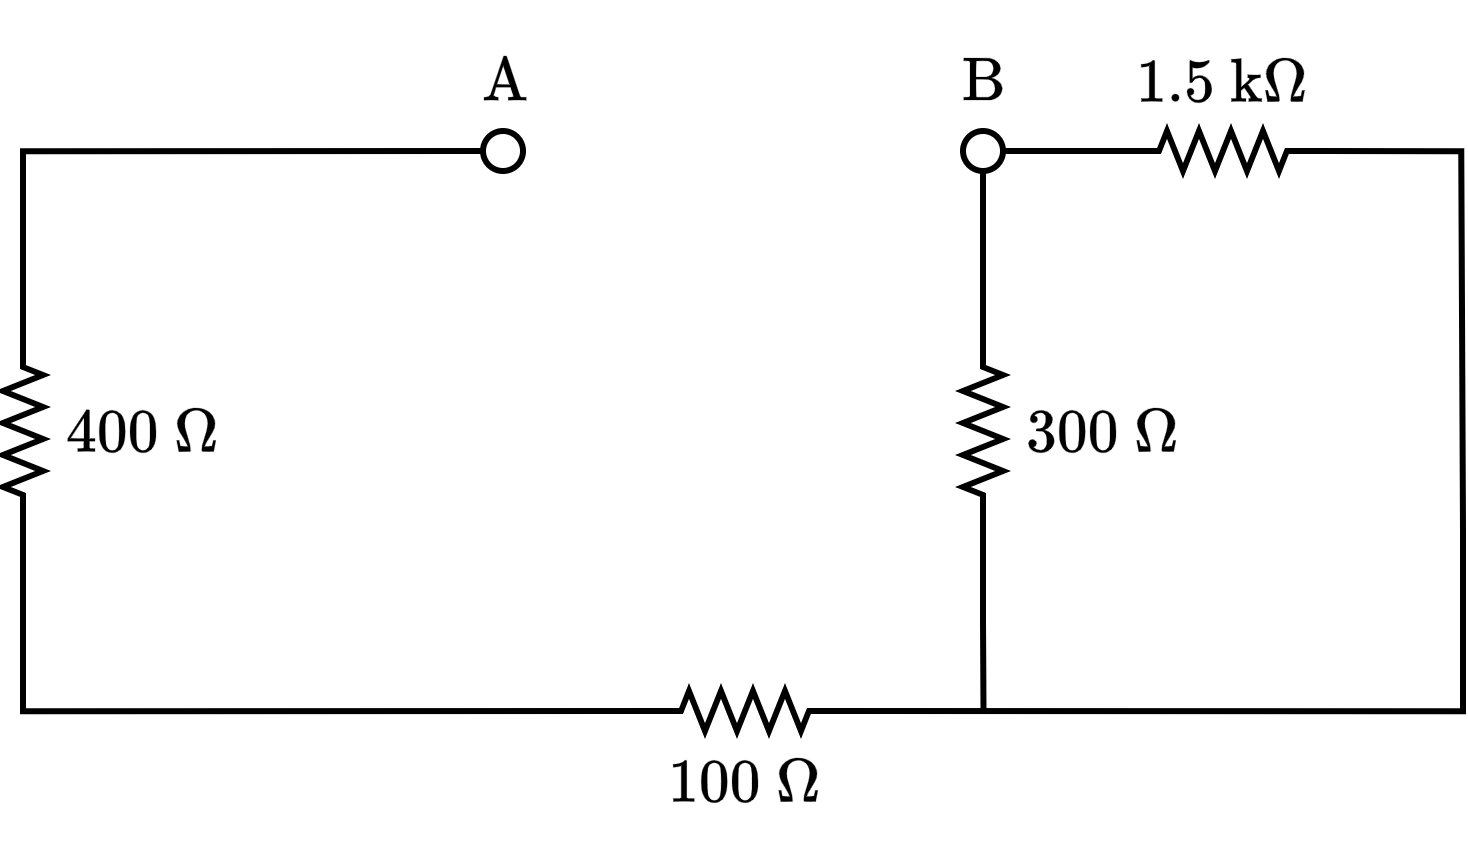
\includegraphics[width=0.7\textwidth]{questionbank/networks/ammeter_thevenin_norton/v1/rthev.png}
\end{center}

We can now combine the remaining resistors to find a single equivalent resistance.

\begin{align*}
    R_{TH} &= \qty{400}{\ohm} + \qty{100}{\ohm} + \qty{300}{\ohm}||\qty{1.5}{\kilo\ohm} \\
    &= \qty{500}{\ohm} + \frac{0.3\cdot1.5}{0.3+1.5}\unit{\kilo\ohm} \\
    &= \qty{750}{\ohm} \\
\end{align*}

\begin{center}
    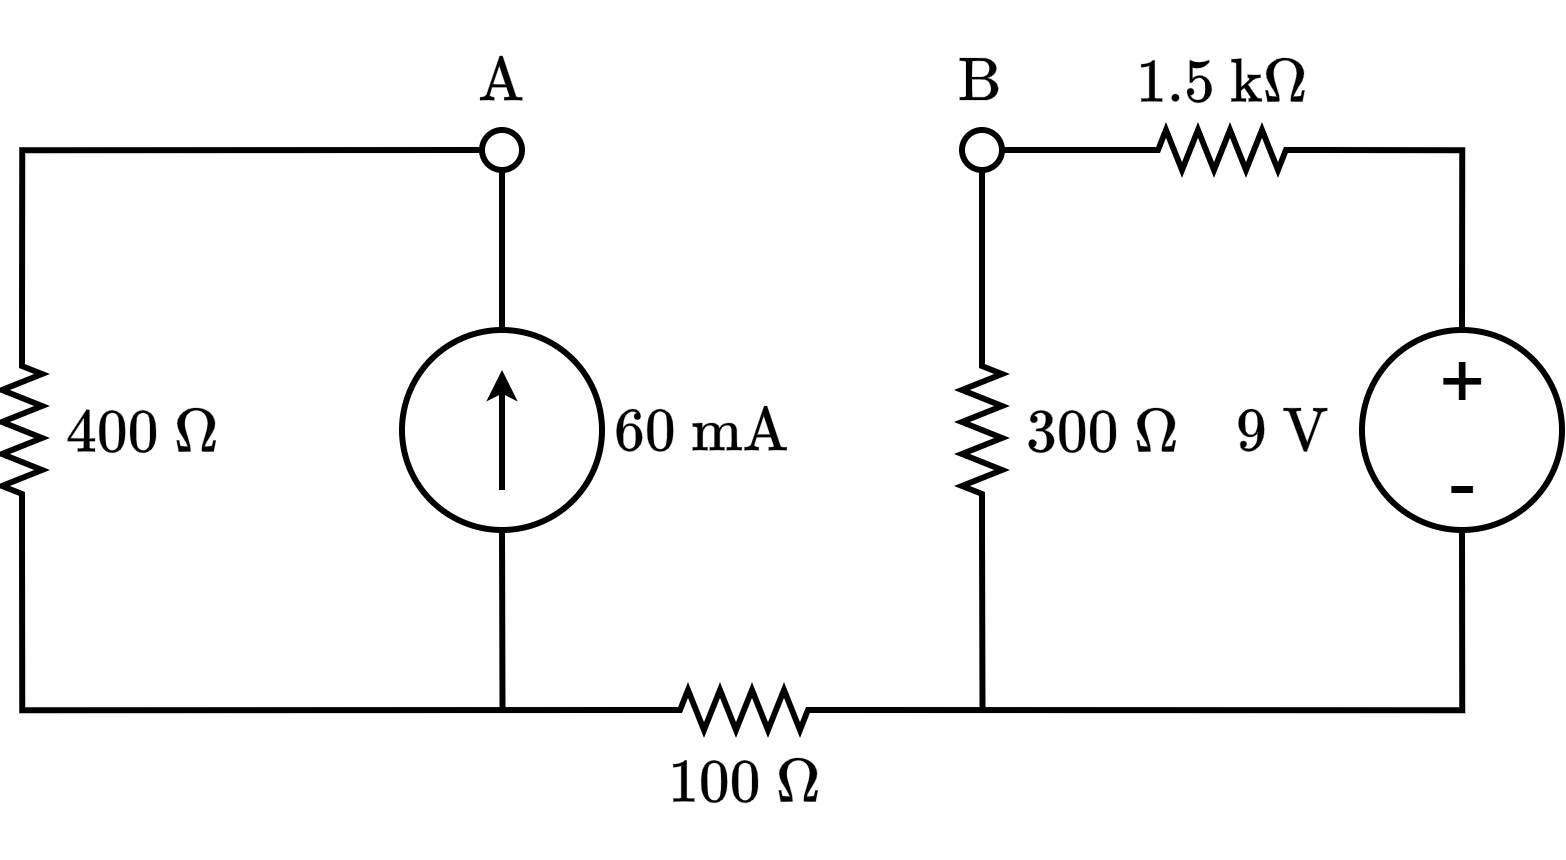
\includegraphics[width=4.5in]{questionbank/networks/ammeter_thevenin_norton/v1/thev_start.png}
\end{center}

Now to find the Thévenin voltage, compute the open-circuit voltage at $A$ and $B$. Because no current flows through the 100$\Omega$ branch, its voltage is zero. The open-circuit voltage measured from $A$ to $B$ is therefore the voltage drop across the current source ($\qty{60}{\milli\ampere} \cdot\qty{400}{\ohm} = \qty{24}{\volt}$) minus the output of the voltage divider formed from the \qty{1.5}{\kilo\ohm} and \qty{300}{\ohm} resistors with the 9 V source ($9 \frac{3}{3+15} = \qty{1.5}{\volt}$). Thus $V_{\text{TH}} = 24 - 1.5 = 22.5~\text{V}$.

Now that we have both the Thévenin voltage and Thévenin resistance, we can combine them to find our equivalent circuit:

\begin{center}
    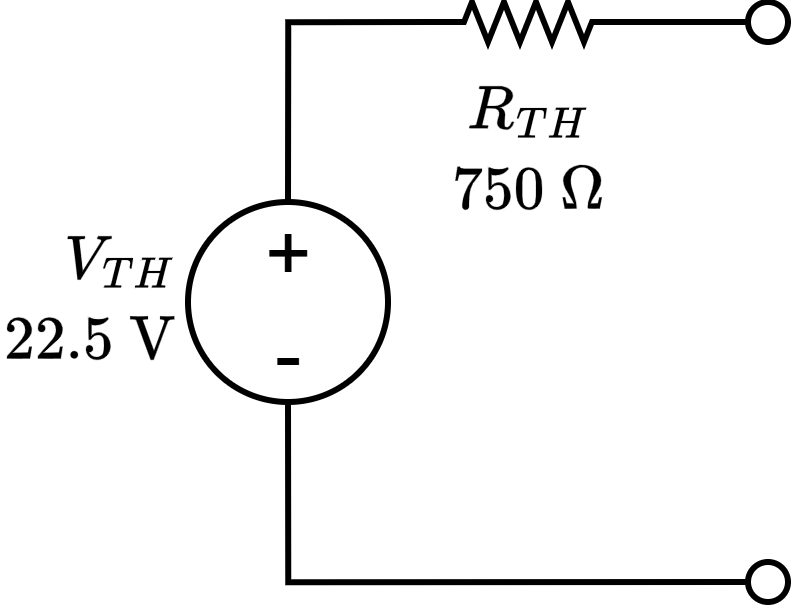
\includegraphics[width=2in]{questionbank/networks/ammeter_thevenin_norton/v1/thev_eq.png}
\end{center}
\end{answer}
\end{partquestion}

\begin{partquestion}{norton}{Find the Norton equivalent circuit at terminals $A$ and $B$ (without the 560$\Omega$ load).}
\begin{answer}
Using the previously computed Thévenin equivalent, the Norton current is $I_{N} = V_{\text{TH}} / R_{\text{TH}} = 22.5~\text{V} / 750~\Omega = 30~\text{mA}$, and $R_{N} = 750\Omega$.

\begin{center}
    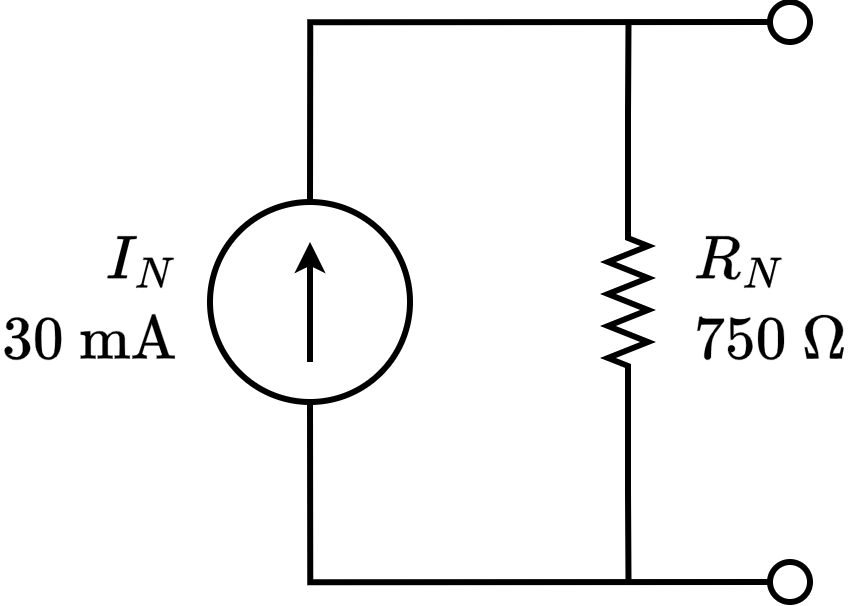
\includegraphics[width=2.2in]{questionbank/networks/ammeter_thevenin_norton/v1/norton_eq.png}
\end{center}
\end{answer}
\end{partquestion}

\begin{partquestion}{ri300}{What is the ammeter reading if $R_{i}=90~\Omega$?}
\begin{answer}
Using the Thévenin equivalent with $R_{i}=90~\Omega$ and $R_{L}=560\Omega$ gives:
\[
I_O = \frac{V_{\text{th}}}{R_{\text{th}} + R_{i} + R_{L}} = \frac{22.5}{750 + 90 + 560} \approx 16.07~\text{mA}.
\]
\end{answer}
\end{partquestion}

\begin{partquestion}{ri0}{What is the ammeter reading if $R_{i}=0~\Omega$?}
\begin{answer}
With $R_{i}=0~\Omega$ the current is:
\[
I_O = \frac{22.5}{750 + 0 + 560} \approx 17.17~\text{mA}.
\]
\end{answer}
\end{partquestion}

\begin{partquestion}{rimax}{What is the maximum value of $R_{i}$ such that the deviation in $I_O$ is less than 1\%? Find the ammeter reading with this maximum.}
\begin{answer}
Let's call the max deviation $\alpha = 0.01$. Since adding any $R_i$ reduces the total current, we wish to determine when $I_{R_i}/I_{0} \geq 1-\alpha$. Let's solve for $R_i$:
\begin{align*}
    \frac{I_{R_i}}{I_0} &\geq 1-\alpha \\
    \frac{R_{th} + R_L}{R_{th} + R_L + R_i} &\geq 1-\alpha \\
    \frac{R_{th} + R_L}{1-\alpha} &\geq R_{th} + R_L + R_i \\
    (R_{th} + R_L)(\frac{1}{1-\alpha} - 1) &\geq R_i \\
    R_i &\leq (R_{th} + R_L)\frac{\alpha}{1-\alpha} \\
    R_i &\leq (750 + 560)\frac{0.01}{0.99} \\
    R_i &\leq 13.23\unit{\ohm}
\end{align*}

Let's find $I_O$ with this new resistance:
\[
I_O = \frac{22.5}{750 + 13.23 + 560} \approx 17.00~\text{mA (nice)}
\]

\end{answer}
\end{partquestion}

\end{mainquestion}


% Problem 4 - Source Transformation Voltage Calculation (18 points)
\clearpage
\Point{sourcetransform}{findvo}{18}
\begin{mainquestion}{sourcetransform}{Source Transformations}
Use source transformations to find the voltage $V_{O}$ in the circuit below.

\begin{center}
    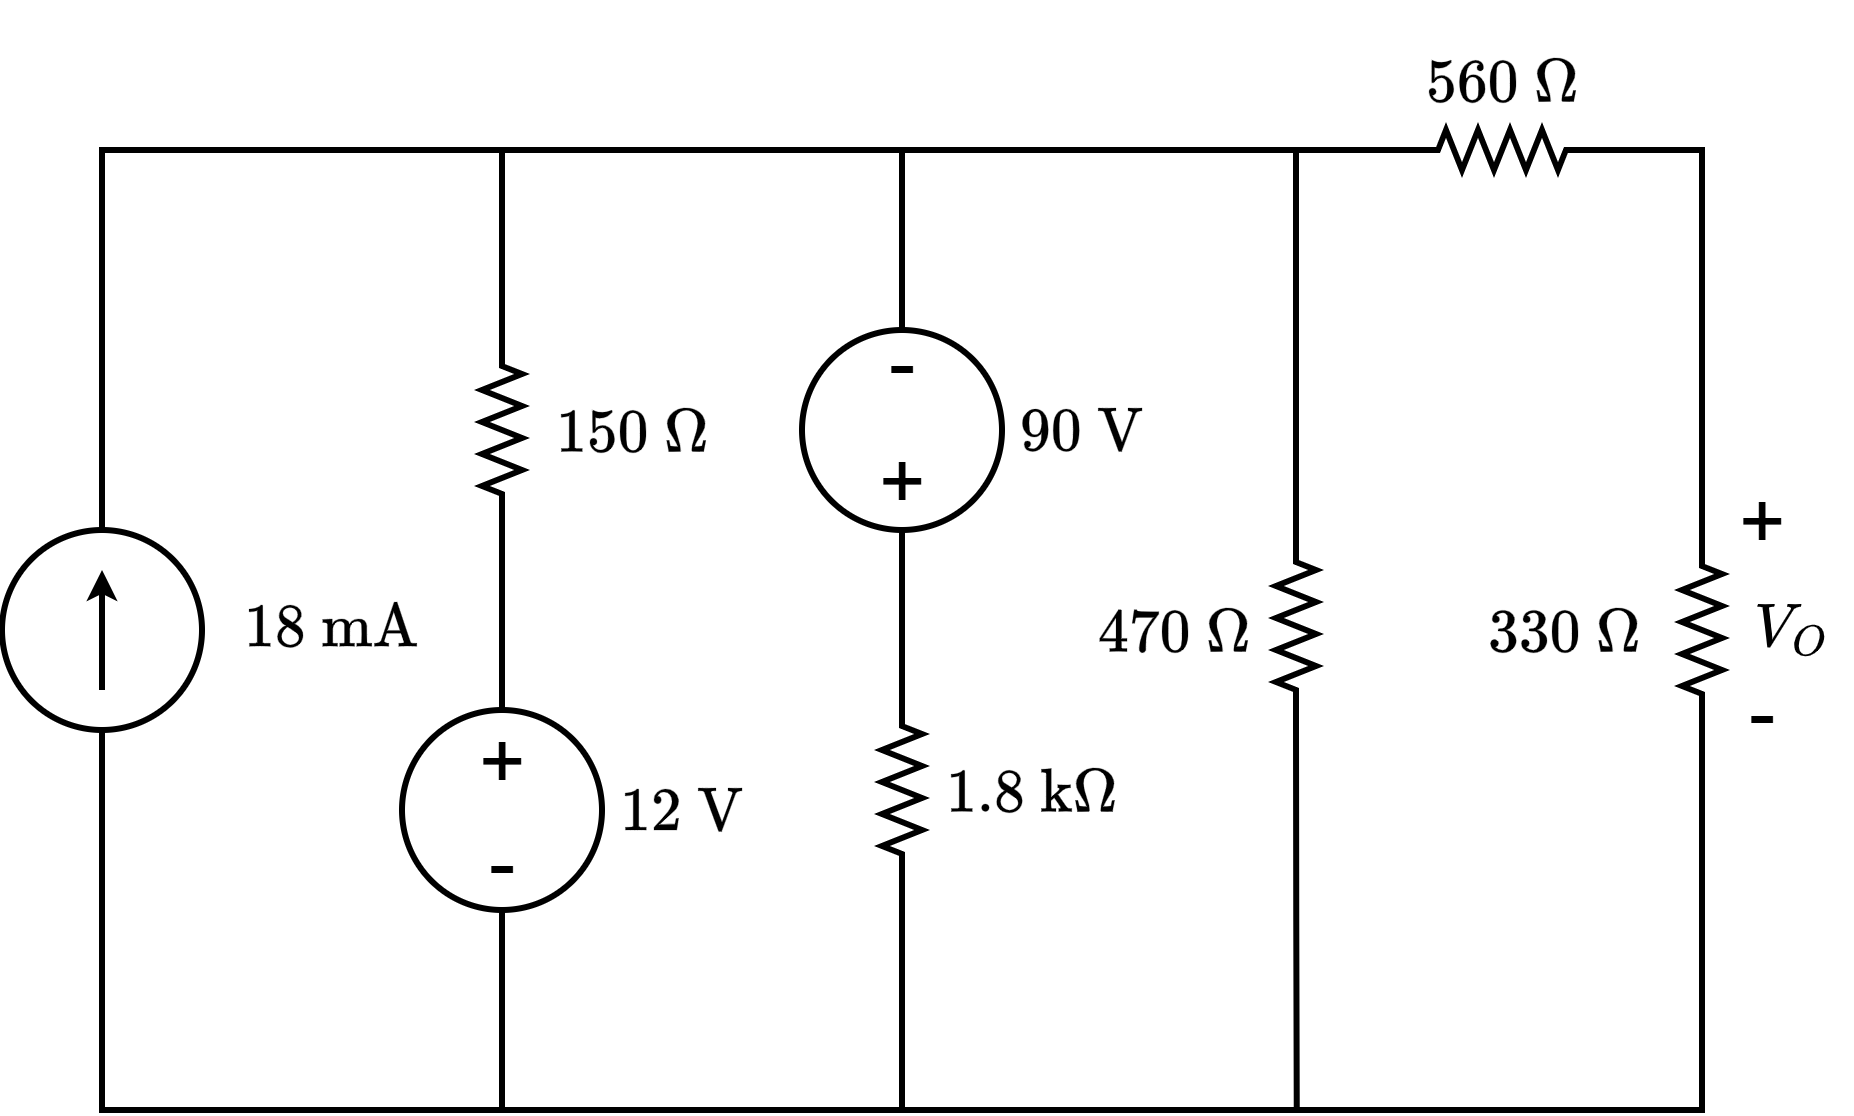
\includegraphics[width=0.8\textwidth]{questionbank/networks/source_transformations/v1/circuit.png}
\end{center}

\begin{partquestion}{findvo}{Find $V_{O}$ using source transformations.}
\begin{answer}
We first transform the 12 V source with the $150~\Omega$ series resistance into its Norton equivalent with a Norton source current of $\frac{\qty{12}{\volt}}{\qty{150}{\ohm}} = \qty{80}{\milli\ampere}$ and a Norton resistance of $150~\Omega$. Simultaneously, we can transform the 90 V source with the \qty{1.8}{\kilo\ohm} series resistance into its Norton equivalent with a Norton source current of $\frac{\qty{90}{\volt}}{\qty{1.8}{\kilo\ohm}} = \qty{50}{\milli\ampere}$ and a Norton resistance of \qty{1.8}{\kilo\ohm}. Note the polarity of the two sources are different, so the Norton current sources will be pointing in different directions! The resulting circuit looks like:

\begin{center}
    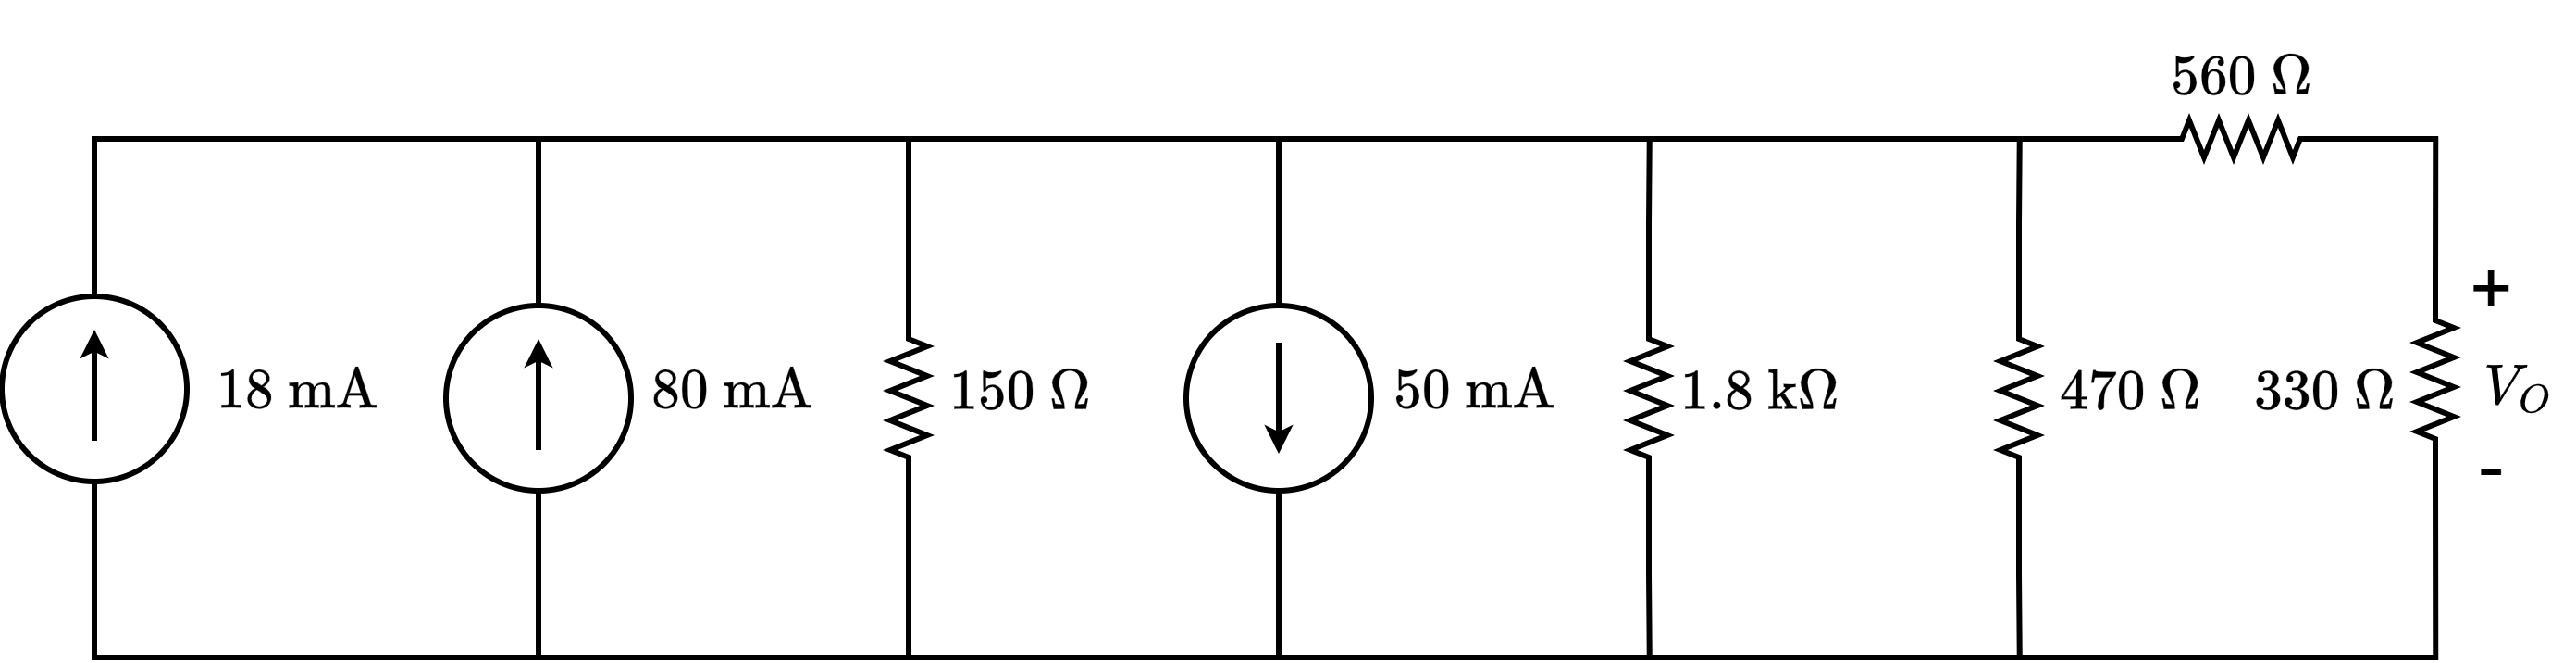
\includegraphics[width=0.8\textwidth]{questionbank/networks/source_transformations/v1/transform_1.png}
\end{center}

We can simplify the circuit considerably by combining the current sources since they are in parallel to form a \qty{48}{\milli\ampere}
source. We can also combine the three parallel resistors with a single resistor of value \qty{107}{\ohm}.
The simplified circuit looks like:

\begin{center}
    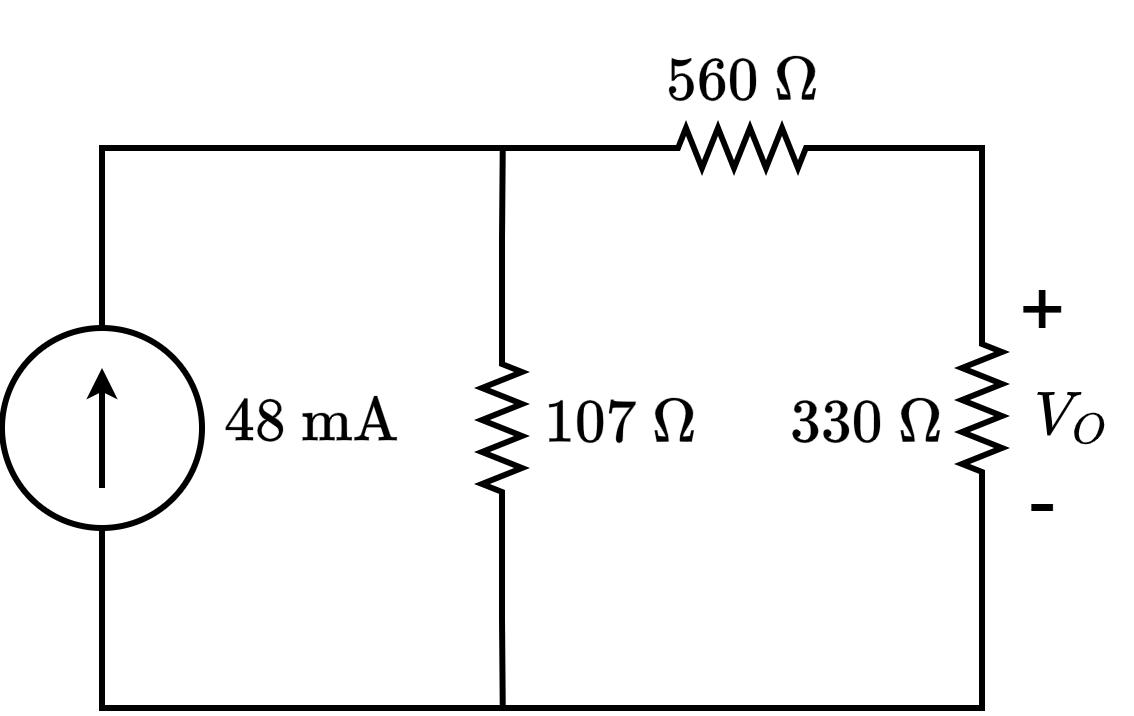
\includegraphics[width=0.5\textwidth]{questionbank/networks/source_transformations/v1/transform_2.png}
\end{center}

The next step is to apply another source transformation to a Thévenin equivalent with a Thévenin voltage source of \qty{5.13}{\volt}
with a Thévenin resistance of \qty{107}{\ohm}.
The result looks like:

\begin{center}
    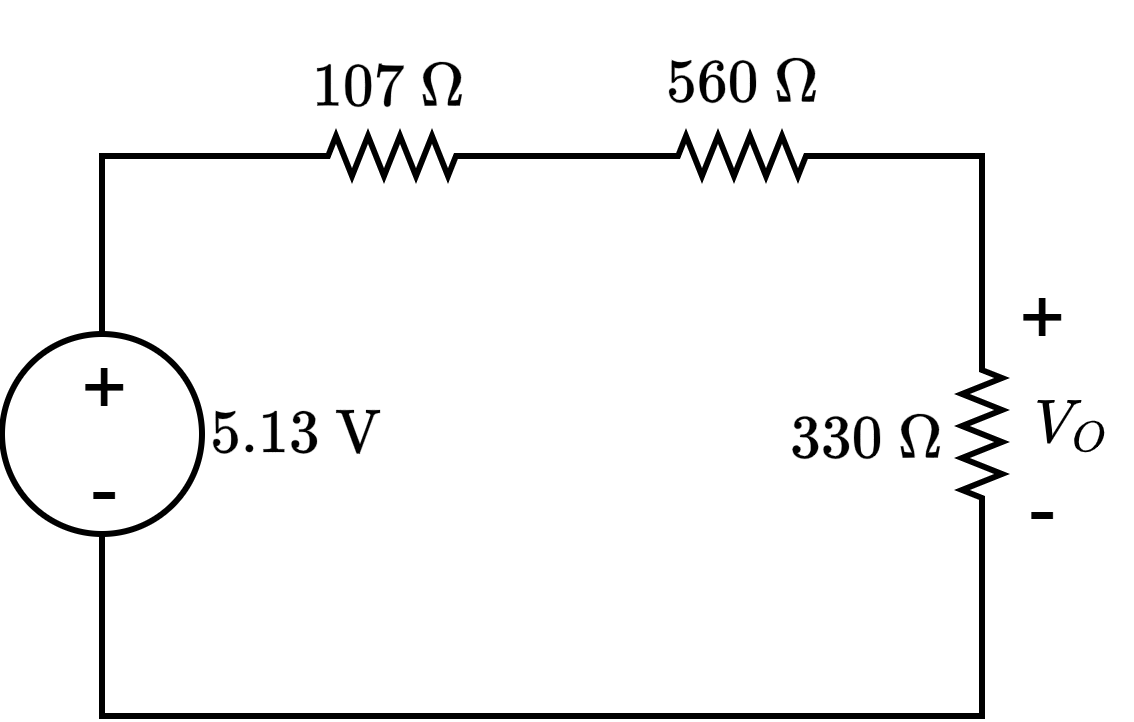
\includegraphics[width=0.5\textwidth]{questionbank/networks/source_transformations/v1/transform_3.png}
\end{center}

The result is a simple voltage divider. We can easily find the voltage across the $330~\Omega$ resistor as:
\[
V_{O}
=
5.13
\left(
\frac{330}{330+560+107}
\right)
=
\qty{1.70}{\volt}
\]
\end{answer}
\end{partquestion}

\end{mainquestion}

% Problem 5 - Your choice (10 points)
\clearpage
\Point{currentgain}{formulavx}{12}
\Point{currentgain}{calculatevx}{2}
\Point{currentgain}{calculatek}{2}
\Point{currentgain}{thev}{5}
\MarkExtraCredit{currentgain}{thev}
\begin{mainquestion}{currentgain}{Your Choice}
Consider the circuit below:

\begin{center}
    \includegraphics[width=0.8\textwidth]{super_cir.png}
\end{center}

\begin{partquestion}{formulavx}{Use a method of your choice to solve for $V_X$ in terms of the current gain $\beta$}
\begin{answer}

Let's evaluate our options. We could use:
\begin{enumerate}
    \item \textbf{Mesh Analysis:} There are 3 meshes, so in the worst worse case we may have 3 KVL equations to solve (If you are familiar with the concept of a supermesh, we could reduce this to one KVL equation)
    \item \textbf{Nodal Analysis:} There are 5 nodes, so in the worst case we may have 4 KCL equations to solve. (If you are familiar with the concept of a supernode, we could reduce this to one KCL equation)
    \item \textbf{Superposition:} There are 3 sources, and we'll have to solve for $V_X$ in the presence of the dependent current source. Worst case three smaller problems.
    \item \textbf{Source Transformations:} Definitely possible, but we'd need to think carefully on how to account for the dependent current source.
\end{enumerate}

Let's use superposition for now given it's a straight forward technique based on our current knowledge. Superposition tells us that we can consider the effect of each independent source individually. We can do this by disabling all but one of the independent sources (open current sources, short voltage sources) and solving for $V_X$. Keep in mind you shouldn't deactivate any dependent sources. Then we can add up all the results and we should get the final value of $V_X$.
\bigskip

\textbf{5 A source only:} short the 10 V and 8V sources. The \qty{4}{\ohm} and \qty{6}{\ohm} resistors can be combined and the whole circuit can be redrawn to look like a current divider as seen below:
\begin{center}
    \includegraphics[width=0.9\textwidth]{super_5A.png}
\end{center}

Let's write our KCL at the top node. $I_X$ can be found with Ohm's law as $I_X = -V_X/10$. Substituting and crunching yields:
\begin{gather*}
0 = \frac{V_X}{2}  - I_X - \beta I_X -5 \\
5 = \frac{V_X}{2} - I_X(1+\beta) \\
5 = \frac{V_X}{2} + V_X\frac{1+\beta}{10} \\
V_X = \frac{5}{\frac{1}{2}+\frac{1+\beta}{10}} = \frac{50}{6+\beta}
\end{gather*}
Let's call this $V_{X\text{,5A}}(\beta)$ and save it for later.
\bigskip

\textbf{8 V source only:} open the 5 A source and short the 10 V source. Combine the resistors as before and the circuit can be rewritten as follows:
\begin{center}
    \includegraphics[width=0.9\textwidth]{super_8V.png}
\end{center}

 This can be solved as before using a KCL equation at the top of the \qty{2}{\ohm} resistor: \[\frac{V_X}{2} - I_X - \beta I_X = 0 \hspace{1cm} I_X = \frac{-8 - V_X}{10}\]
 Solving...
\begin{gather*}
\frac{V_X}{2} - I_X(1+\beta)= 0 \\
\frac{V_X}{2} +\frac{8 + V_X}{10}(1+\beta)= 0 \\
V_X\left(\frac{1}{2} + \frac{(1+\beta)}{10}\right) = -\frac{8(1+\beta)}{10} \\
V_X = \frac{-\frac{8(1+\beta)}{10}}{\frac{1}{2} + \frac{(1+\beta)}{10}} = \frac{-8(1+\beta)}{6+\beta}
\end{gather*}
Let's call this $V_{X\text{,8V}}(\beta)$ and save it for later.
\bigskip

\textbf{10 V source only:} open the 5 A source and short the 8 V source. Combine the resistors as before and the circuit can be rewritten as follows:
\begin{center}
    \includegraphics[width=0.9\textwidth]{super_10V.png}
\end{center}

This can be solved as before using a KCL equation at the top of the \qty{2}{\ohm} resistor: \[\frac{V_X}{2} - I_X - \beta I_X = 0 \hspace{1cm} I_X = \frac{-10 - V_X}{10}\]
Note that this is the same as the \qty{8}{\volt} equation except we are using \qty{-10}{\volt} instead. Replacing the voltage leads to...
\begin{gather*}
V_X\left(\frac{1}{2} + \frac{(1+\beta)}{10}\right) = -\frac{10(1+\beta)}{10} \\
V_X = \frac{-(1+\beta)}{\frac{1}{2} + \frac{(1+\beta)}{10}} = \frac{-10(1+\beta)}{6+\beta}
\end{gather*}
Let's call this $V_{X\text{,10V}}(\beta)$ and save it for later.
\bigskip
 
\textbf{Summation:}

Superposition tells us the final solutions is the addition of all three functions we derived:
\begin{align*}
V_X(\beta) &= V_{X\text{,5A}}(\beta) + V_{X\text{,8V}}(\beta) + V_{X\text{,10V}}(\beta) \\
V_X(\beta)&= \frac{50}{6+\beta} + \frac{-8(1+\beta)}{6+\beta} + \frac{-10(1+\beta)}{6+\beta} \\
V_X(\beta)&= \frac{50 - 18(1+\beta)}{6+\beta} = \frac{32 - 18\beta}{6+\beta}
\end{align*}
\end{answer}
\end{partquestion}

\begin{partquestion}{calculatevx}{Solve for $V_X$ given that $\beta = 0.25$}
\begin{answer}
Finding this is as simple as plugging in the given value of $\beta$.
\begin{align*}
    V_X(0.25)&= \frac{32 - 18\cdot0.25}{6+0.25} = \qty{4.4}{\volt}
\end{align*}
\end{answer}
\end{partquestion}

\begin{partquestion}{calculatek}{Find $\beta$ such that $V_X = \qty{17}{\volt}$}
\begin{answer}
This will require flipping the equation around to solve for $\beta$.
\begin{align*}
    V_X &= \frac{32 - 18\beta}{6+\beta} \\
    V_X(6+\beta) &= 32 - 18\beta \\
    \beta(18 + V_X) &= 32 - 6V_X \\
    \beta &= \frac{32 - 6V_X}{18 + V_X} \\
    \beta &= \frac{32 - 6\cdot17}{18 + 17} = -2 \\
\end{align*}
\end{answer}
\end{partquestion}

\begin{partquestion}{thev}{Find the equivalent resistance seen across $V_X$ in terms of $\beta$. What happens when $\beta = -6$? Use this to explain the result of $V_X(-6)$ from part (\cref{prob:currentgain:formulavx}).}

\begin{answer}
    We can find $R_{th}$ by disabling all independent sources and applying a test voltage and measuring the current that flows out of it. The ratio between these is the equivalent resistance! Since we are asked to find the equivalent resistance across $V_X$, we will attach our test source in parallel.
\begin{center}
    \includegraphics[width=0.9\textwidth]{rth.png}
\end{center}

Let's solve for $I_T$ using a KCL equation. Recall $V_X = V_T$.
\begin{align*}
    \frac{V_X}{2} - I_X - \beta I_X &= I_T \\
    \frac{V_T}{2} - I_X(1+\beta) &= I_T \\
    \frac{V_T}{2} - \left(-\frac{V_T}{10}\right)(1+\beta) &= I_T \\
    V_T\left(\frac{1}{2} + \frac{1+\beta}{10}\right) &= I_T \\
\end{align*}
We can then find $R_{th} = V_T/I_T$:
\begin{align*}
    R_{th} = \frac{V_T}{I_T} &= \frac{1}{\frac{1}{2} + \frac{1+\beta}{10}} \\
    R_{th} &= \frac{10}{5 + (1+\beta)} \\
    R_{th} &= \frac{10}{6+\beta} \\
\end{align*}
We have now found the equivalent resistance in terms of the current gain $\beta$. When the current gain $\beta = -6$, the formula predicts $R_{th} = \infty$, an open circuit. The dependent current source provides just enough current to satisfy the \qty{10}{\ohm} and \qty{2}{\ohm} resistor at any voltage, so there isn't any room for an ideal source to supply or draw any additional current $I_T$. The formula from part (\cref{prob:currentgain:formulavx}):
\[
V_X = \frac{32 - 18\beta}{6+\beta}
\]
shows that $V_X$ also blows up to infinity when $\beta = -6$. This makes senses because we have a \qty{5}{\ampere} source trying to drive current into our open load. Ohm's law suggests $V = I\cdot R$, so $V_X = 5 \cdot \infty = \infty$.
    
\end{answer}
\end{partquestion}

\end{mainquestion}


% Problem 6 - Battery Internal Resistance and Power Curve (10 points)
\clearpage
\Point{battery}{peakcurrent}{2}
\Point{battery}{peakpower}{4}
\Point{battery}{plotpower}{4}
\begin{mainquestion}{battery}{Power Transfer}
A typical CR2032 3 V coin-style battery (often used in watches or small electronic devices) has an internal source resistance $R_{s}$ of about $17~\si{\ohm}$ (seriously!) at room temperature. (While this value typically increases as the battery is depleted, we will consider it constant for this problem.)

\begin{center}
    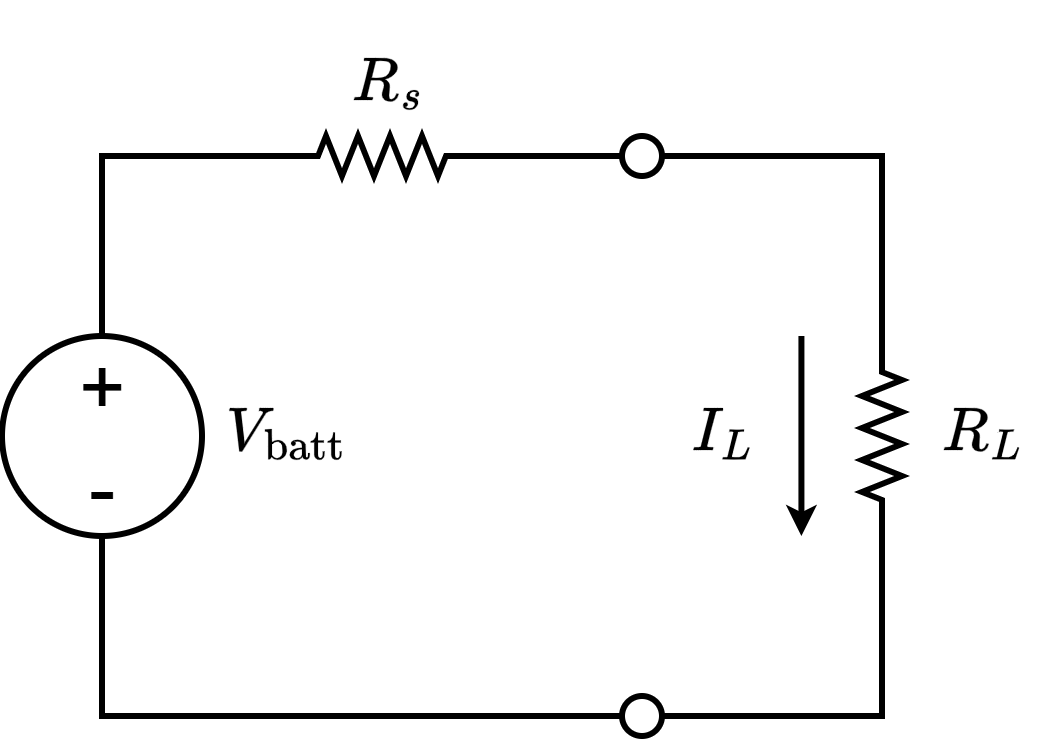
\includegraphics[width=4in]{questionbank/networks/battery_internal_resistance/v0/circuit.png
    }
\end{center}

\begin{partquestion}{peakcurrent}{Using this battery, what is the peak current that could be driven through an external load $R_{L}$? What is $R_{L}$ in this scenario?}
\begin{answer}
The current is
\[
I=\frac{V_{\text{batt}}}{R_s+R_L},
\]
and to make this as large as possible, we make the denominator as small as possible. With $R_s$ fixed, we make
\[
R_L=0,
\]
so
\[
I=\frac{V_{\text{batt}}}{R_s} = \frac{3}{17}\,\si{\ampere}
    \approx 176\,\si{\milli\ampere}.
\]
\end{answer}
\end{partquestion}

\begin{partquestion}{peakpower}{Using this battery, what is the peak power that could be delivered through an external load $R_{L}$? What is $R_{L}$ in this scenario?}
\begin{answer}
Maximum power transfer occurs when
\[
R_L=R_s=17\,\si{\ohm},
\]
and the value of the power is
\[
P= \frac{V_L^2}{R_L} = \frac{(V_{\text{batt}}\frac{R_L}{R_s + R_L})^2}{R_L} = \frac{V_{\text{batt}}^2R_L}{(R_s + R_L)^2}
= \frac{V_{\text{batt}}^2}{4R_s}
=\frac{3^2}{4(17)}
=\frac{9}{68}\,\si{\watt}
\approx132\,\si{\milli\watt}.
\]
\end{answer}
\end{partquestion}

\begin{partquestion}{plotpower}{Plot the power delivered to $R_{L}$ as a function of $R_{L}$, from $0$ to $500~\si{\ohm}$.}
\begin{answer}
In the previous part, we derived the formula for the power dissipated in the load as:
\[P_{L} = \frac{V_{\text{batt}}^{2} R_{L}}{(R_{L} + R_{s})^{2}} = \frac{9 R_{L}}{(R_{L} + 17)^{2}}.\]

This can be plotted using MATLAB or some equivalent graphing program; the figure is shown below.

\begin{center}
    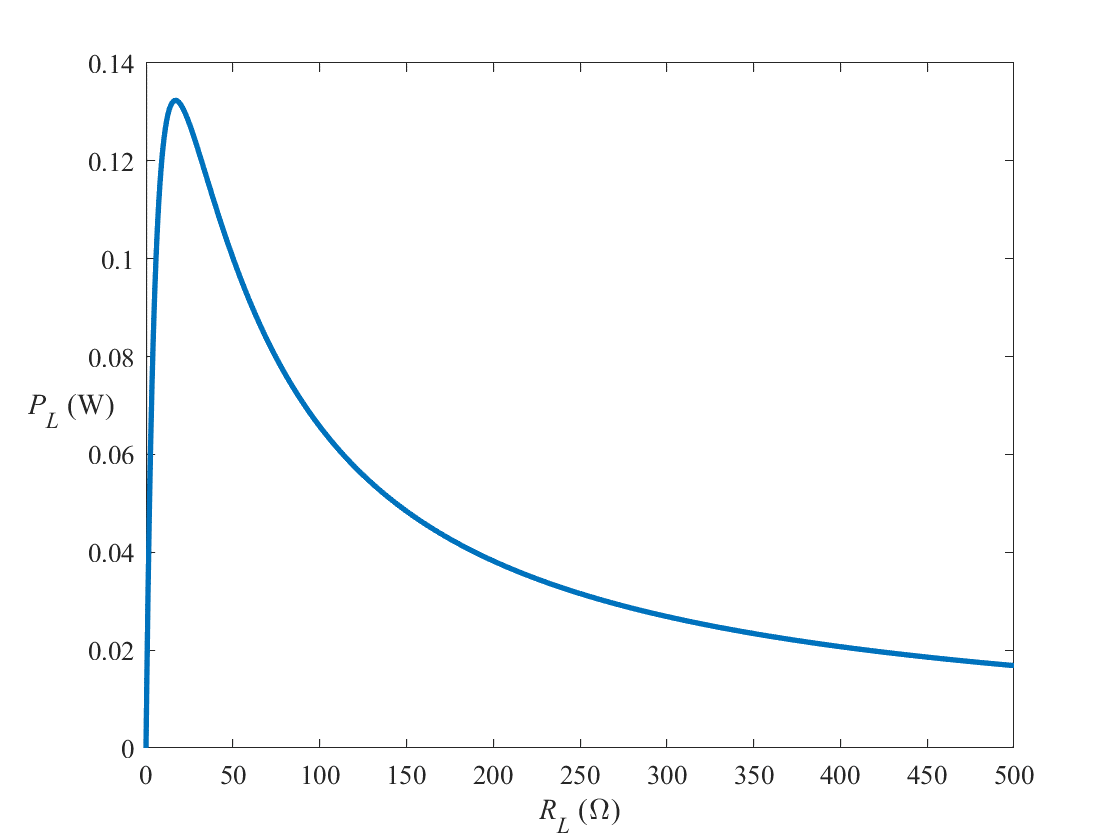
\includegraphics[width=5in]{questionbank/networks/battery_internal_resistance/v0/plot.png}
\end{center}

Note the peak occurs at $17~\si{\ohm}$, as we expect. The power delivered to the load rolls off to zero as $R_L$ goes to zero.
\end{answer}
\end{partquestion}

\end{mainquestion}
